\begin{frame}
    \frametitle{Variables}
    \begin{itemize}
        \item Mesh size
        \item Periodic load: \begin{itemize}
            \item Frequency
            \item Amplitude
            \item Duration
        \end{itemize}

            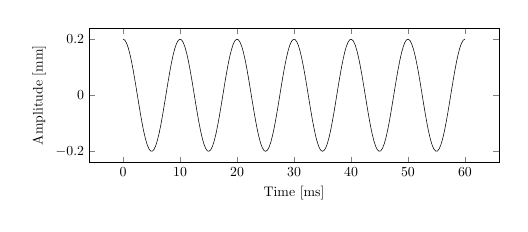
\begin{tikzpicture}[scale=0.5]
                \begin{axis}[width=12cm, height = 5cm,
                    xlabel = {Time [ms]}, ylabel = {Amplitude [mm]},
                    ]
                    \addplot[no marks, domain=0:60, samples = 200,] {0.2*cos(2*pi*0.1*deg(x))};
                \end{axis}
            \end{tikzpicture}
        \item Position of load
        
    \end{itemize}
    
\end{frame}

\begin{frame}
    \frametitle{Modal analysis}

    \begin{itemize}
        \item Ensure ITAP is well-behaved in the clinically important frequency range
        \item Define the frequency bounds for our simulations
    \end{itemize}
    \begin{columns}
        \begin{column}{0.5\textwidth} \centering
            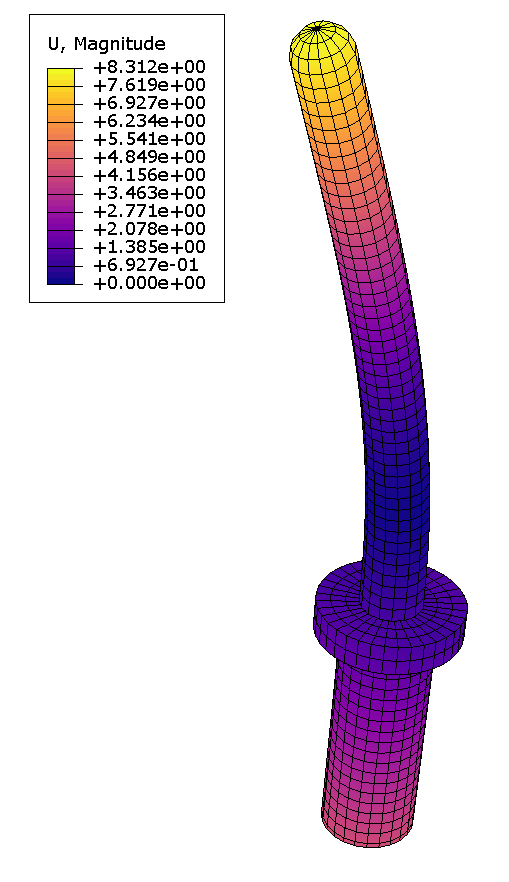
\includegraphics[height=4cm]{../figures/934.png}

            \textbf{12cm stem: 930 Hz}
        \end{column}
        \begin{column}{0.5\textwidth} \centering
            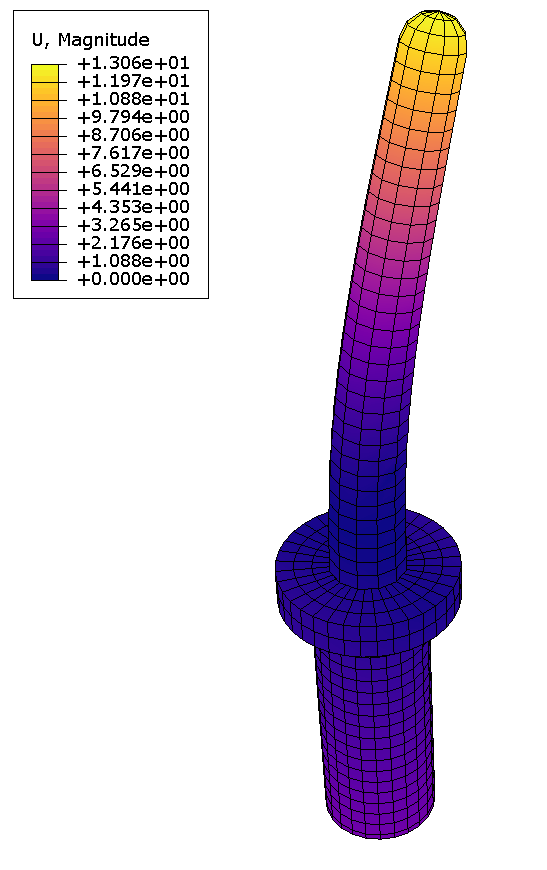
\includegraphics[height=4cm]{figures/8cm-1668hz resonance.png}

            8cm stem: 1670 Hz
        \end{column}
    \end{columns}

\end{frame}